% Generated by `uv run analyze`; needs \usepackage{pgfplots}
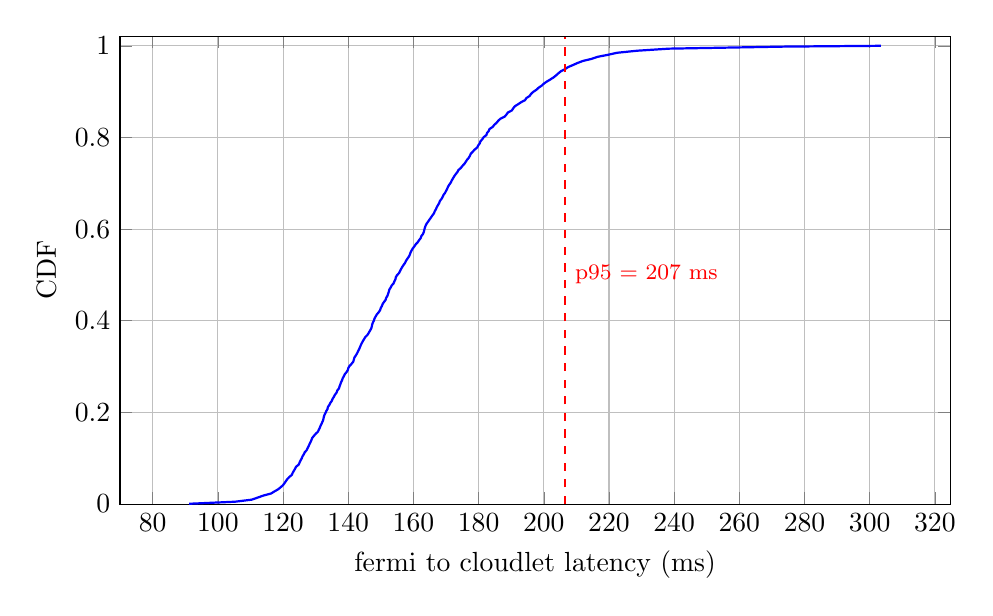
\begin{tikzpicture}
\begin{axis}[xlabel={fermi to cloudlet latency (ms)}, ylabel={CDF}, width=\columnwidth, height=0.62\columnwidth, grid=major, ymin=0, ymax=1.02]
\addplot[thick, blue] coordinates {(91.179,0.0006) (105.258,0.0051) (110.392,0.0096) (112.173,0.0140) (113.926,0.0185) (116.307,0.0230) (117.336,0.0275) (118.454,0.0320) (119.238,0.0365) (119.947,0.0410) (120.445,0.0455) (120.853,0.0500) (121.315,0.0545) (121.908,0.0590) (122.663,0.0635) (122.946,0.0680) (123.306,0.0725) (123.691,0.0770) (124.003,0.0815) (124.791,0.0860) (125.059,0.0904) (125.349,0.0949) (125.704,0.0994) (125.955,0.1039) (126.353,0.1084) (126.64,0.1129) (127.225,0.1174) (127.533,0.1219) (127.83,0.1264) (128.131,0.1309) (128.436,0.1354) (128.72,0.1399) (128.958,0.1444) (129.477,0.1489) (130.03,0.1534) (130.7,0.1579) (130.979,0.1624) (131.288,0.1669) (131.531,0.1713) (131.844,0.1758) (132.134,0.1803) (132.348,0.1848) (132.475,0.1893) (132.663,0.1938) (132.988,0.1983) (133.254,0.2028) (133.634,0.2073) (133.75,0.2118) (134.203,0.2163) (134.52,0.2208) (134.963,0.2253) (135.199,0.2298) (135.616,0.2343) (135.95,0.2388) (136.435,0.2433) (136.634,0.2478) (137.143,0.2522) (137.321,0.2567) (137.581,0.2612) (137.786,0.2657) (138.101,0.2702) (138.314,0.2747) (138.667,0.2792) (138.97,0.2837) (139.505,0.2882) (139.878,0.2927) (140.037,0.2972) (140.441,0.3017) (141.05,0.3062) (141.531,0.3107) (141.72,0.3152) (141.895,0.3197) (142.315,0.3242) (142.7,0.3287) (142.994,0.3331) (143.306,0.3376) (143.588,0.3421) (143.841,0.3466) (144.149,0.3511) (144.485,0.3556) (144.871,0.3601) (145.251,0.3646) (145.894,0.3691) (146.291,0.3736) (146.638,0.3781) (147.02,0.3826) (147.215,0.3871) (147.339,0.3916) (147.549,0.3961) (147.877,0.4006) (148.081,0.4051) (148.425,0.4096) (148.791,0.4140) (149.333,0.4185) (149.762,0.4230) (149.963,0.4275) (150.31,0.4320) (150.546,0.4365) (150.976,0.4410) (151.451,0.4455) (151.644,0.4500) (152.037,0.4545) (152.232,0.4590) (152.454,0.4635) (152.612,0.4680) (153.016,0.4725) (153.317,0.4770) (153.906,0.4815) (154.156,0.4860) (154.473,0.4904) (154.597,0.4949) (154.961,0.4994) (155.571,0.5039) (155.896,0.5084) (156.206,0.5129) (156.567,0.5174) (156.979,0.5219) (157.446,0.5264) (157.717,0.5309) (158.139,0.5354) (158.597,0.5399) (158.898,0.5444) (159.117,0.5489) (159.441,0.5534) (159.8,0.5579) (160.298,0.5624) (160.72,0.5669) (161.308,0.5713) (161.724,0.5758) (162.226,0.5803) (162.43,0.5848) (162.926,0.5893) (163.18,0.5938) (163.344,0.5983) (163.495,0.6028) (163.732,0.6073) (164.041,0.6118) (164.506,0.6163) (164.924,0.6208) (165.383,0.6253) (165.812,0.6298) (166.289,0.6343) (166.526,0.6388) (166.894,0.6433) (167.164,0.6478) (167.514,0.6522) (167.899,0.6567) (168.101,0.6612) (168.604,0.6657) (168.965,0.6702) (169.238,0.6747) (169.715,0.6792) (170.034,0.6837) (170.364,0.6882) (170.625,0.6927) (171.02,0.6972) (171.478,0.7017) (171.76,0.7062) (172.139,0.7107) (172.505,0.7152) (172.956,0.7197) (173.464,0.7242) (173.774,0.7287) (174.511,0.7331) (174.989,0.7376) (175.603,0.7421) (176.025,0.7466) (176.438,0.7511) (176.972,0.7556) (177.342,0.7601) (177.606,0.7646) (178.222,0.7691) (178.796,0.7736) (179.573,0.7781) (179.892,0.7826) (180.339,0.7871) (180.573,0.7916) (181.132,0.7961) (181.541,0.8006) (182.368,0.8051) (182.576,0.8096) (183.083,0.8140) (183.363,0.8185) (184.321,0.8230) (184.8,0.8275) (185.511,0.8320) (186.033,0.8365) (186.7,0.8410) (187.996,0.8455) (188.545,0.8500) (188.984,0.8545) (190.206,0.8590) (190.608,0.8635) (191.108,0.8680) (192.103,0.8725) (193.071,0.8770) (194.259,0.8815) (194.655,0.8860) (195.635,0.8904) (196.066,0.8949) (196.748,0.8994) (197.707,0.9039) (198.386,0.9084) (199.33,0.9129) (200.011,0.9174) (200.918,0.9219) (201.969,0.9264) (202.965,0.9309) (203.76,0.9354) (204.458,0.9399) (205.234,0.9444) (206.446,0.9489) (207.413,0.9534) (208.9,0.9579) (210.325,0.9624) (211.973,0.9669) (214.573,0.9713) (216.418,0.9758) (219.628,0.9803) (222.494,0.9848) (228.695,0.9893) (238.456,0.9938) (274.129,0.9983) (303.461,1.0000)};
\draw[red, dashed, thick] (axis cs:206.604,0) -- (axis cs:206.604,1.02);
\node[red, anchor=west, font=\footnotesize] at (axis cs:206.604,0.5) {p95 = 207 ms};
\end{axis}
\end{tikzpicture}
